\documentclass[12pt,a4paper]{article}
\usepackage[utf8]{inputenc}
\usepackage{ngerman}
\usepackage{amsmath}
\usepackage{amsfonts}
\usepackage{amssymb}
\usepackage{graphicx}
\usepackage{color}
\usepackage{enumerate}
\usepackage{lineno}
\usepackage{listings} 
\definecolor{lightgrey}{rgb}{0.90,0.90,0.90}
\lstset{language=Java, backgroundcolor=\color{lightgrey},  numbersep=5pt, tabsize=3}

\setlength{\parindent}{0em}
\setlength{\parskip}{0.5em}

\title{Lösungsstrategien für NP-schwere Probleme\\Blatt 9}
\author{
		Jakob Rieck\\
		\small{6423721}
	\and
		Konstantin Kobs\\
		\small{6414943}
	\and
		Thomas Maier\\
		\small{6319878}
	\and
		Tom Petersen\\
		\small{6359640}
}
\date{Abgabe zum 27.06.16}


\begin{document}

\maketitle

\section*{Aufgabe 1}

\begin{enumerate}[a)]
	\item Im Folgenden werden wir lediglich in Anteilen der Gesamtrechenpower sprechen. So ist beispielsweise $T_1 = \frac{1}{3}$ eine Abkürzung für $T_1 = \frac{1}{3} \sum_{i=1}^{n} t_i$.\\
		Die angegebene Bedingung sagt nun aus, dass sich sowohl $T_1$ als auch $T_2$ zwischen $\frac{1}{3}$ und $\frac{2}{3}$ aufhalten, denn $T_1 + T_2 = 1$. Zu zeigen ist also, dass wann immer die beiden $T$ außerhalb dieser Schranken sind, eine Möglichkeit besteht, ein $t_i$ aus der stärker belasteten auf die weniger belastete Maschine zu übertragen. Ist dies nicht mehr möglich, so sind beide Maschinen ausgeglichen genug (nach den gewünschten Ungleichungen).\\
		Wir nehmen nun an, dass die erste Maschine eine Auslastung $T_1 \geq \frac{2}{3}$ hat, wodurch die andere Maschine eine Auslastung von $T_2 = 1 - T_1 \leq \frac{1}{3}$ besitzt. Der Beweis für den umgekehrten Fall geht dann analog. Aufgrund der Nicht-Dominanz-Bedingung muss gelten, dass Maschine 1 aus mindestens zwei Prozessen besteht. Ein Umschaufeln der Prozesse kann nur dann ausgeführt werden, wenn $|T_1 - T_2|$ mit diesem Übertragen kleiner wird. Damit dies kleiner wird, kann maximal ein Prozess von Maschine 1 zu Maschine 2 übertragen werden, denn ein umgekehrtes Übertragen würde die absolute Differenz der beiden Maschinen-Auslastungen zunächst steigern, was im gewünschten Ansatz nicht zulässig ist. Damit also eine Übertragung möglich ist, muss mindestens ein Prozess von Maschine 1 kleiner sein als die absolute Differenz der beiden Maschinen, denn nur so kann ein Sinken der Differenz gewährleistet werden. Wir schauen uns im Folgenden nur den kleinsten Prozess von Maschine an, denn dieser kann im Falle einer möglichen Übertragung auf jeden Fall übertragen werden. Seien nun $k$ Prozesse Maschine zugeordnet. Dann ist der kleinste Prozess dieser Maschine maximal $\frac{1}{k} \cdot T_1$ groß. Der größte kleinste Prozess, der jemals erreicht werden kann, ist wenn $k=2$ gilt. Der Prozess ist dann maximal $\frac{1}{2} \cdot T_1$ groß, und weil $T_1 \geq \frac{2}{3}$ gilt, muss der kleinste Prozess $t_{1,min}$ zwischen $\frac{1}{6}$ und $\frac{1}{3}$ liegen. Ist $k$ größer als zwei, so hat der kleinste Prozess einen geringeren Minimal-Wert. Wenn wir nun $t_{1,min}$ auf Maschine 2 umschaufeln würden, so hätte nach dem Tauschen Maschine 1 eine Auslastung zwischen $\frac{1}{3}$ und $\frac{1}{2}$. Maschine 2 hat dann eine Auslastung zwischen $\frac{1}{2}$ und $\frac{2}{3}$, da $T_2 = 1 - T_1$ gilt und somit, je größer $T_1$ ist, $T_2$ kleiner wird.\\
		Beide Maschinen-Auslastungen erfüllen nun die Ungleichungen, die als Bedingung erfordert waren. Für ein größeres $k$ kann es sein, dass der kleinste Prozess kleiner ist und die Auslastungen noch außerhalb der Grenzen der Ungleichungen. Allerdings gilt dann nach einem Umschaufeln des kleinsten Prozesses weiterhin die Voraussetzung, mit der ein weiteres Umschaufeln ermöglicht wird. Somit landen wir immer in den angestrebten Grenzen. Zu Bemerken ist allerdings noch, dass auch ein Tausch möglich sein kann, selbst wenn beide Maschinen in den Grenzen liegen. Dies ist aber okay, da mit einem Tausch die Grenzen nicht erneut überschritten werden können. $\square$

	\item Die absolute Differenz der beiden Auslastungen $|T_1 - T_2|$ wird mit jedem Tausch immer kleiner. Bei der Strategie mit dem größten Prozess, der von der höher ausgelasteten Maschine zur weniger ausgelasteten Maschine übertragen wird, wird immer der Prozess ausgewählt, der so groß wie möglich, aber immer noch kleiner als $|T_1 - T_2|$ ist, da sonst diese Differenz nicht verkleinert werden kann. Wird nun ein Prozess nach der Strategie ausgewählt und übertragen, so wird die absolute Differenz der beiden Auslastungen kleiner als die Größe des übertragenen Prozesses. Da in jedem Schritt die Differenz immer kleiner werden muss, gibt es somit keine Möglichkeit mehr, dass der ausgewählte Prozess erneut ausgewählt wird. $\square$
		
	\item Seien beide Maschinen mit folgenden Jobs $t_1, t_2, t_3, t_4$ initialisiert: Maschine 1 enthält die Prozesse $t_1 = 1, t_2 = 2, t_3 = 3$ und Maschine 2 den Prozess $t_4 = 3,99$. Somit ist also $T_1 = 6$ und $T_2 = 3,99$. Zum Verschieben kommen die Jobs $t_1$ und $t_2$ infrage, da $|T_1 - T_2| = 2,01$ ist und diese absolute Differenz durch Verschiebung von $t_1$ auf $0,01$ und durch Verschiebung von $t_2$ auf $1,99$ verringert werden kann. Die Regel aus b) besagt nun, dass der Prozess mit der größten Auslastung ausgewählt wird. Das ist in diesem Fall $t_2$, wobei jedoch $t_1$ einen sehr viel besseren Score liefert. Beide Schritte würden zu einer Lösung führen, die das Verschieben von Prozessen abbricht, jedoch führt der gewählte Schritt nicht zur optimalen Lösung.
		
\end{enumerate}



\section*{Aufgabe 2}

	\begin{figure}%[ht]
		\centering
		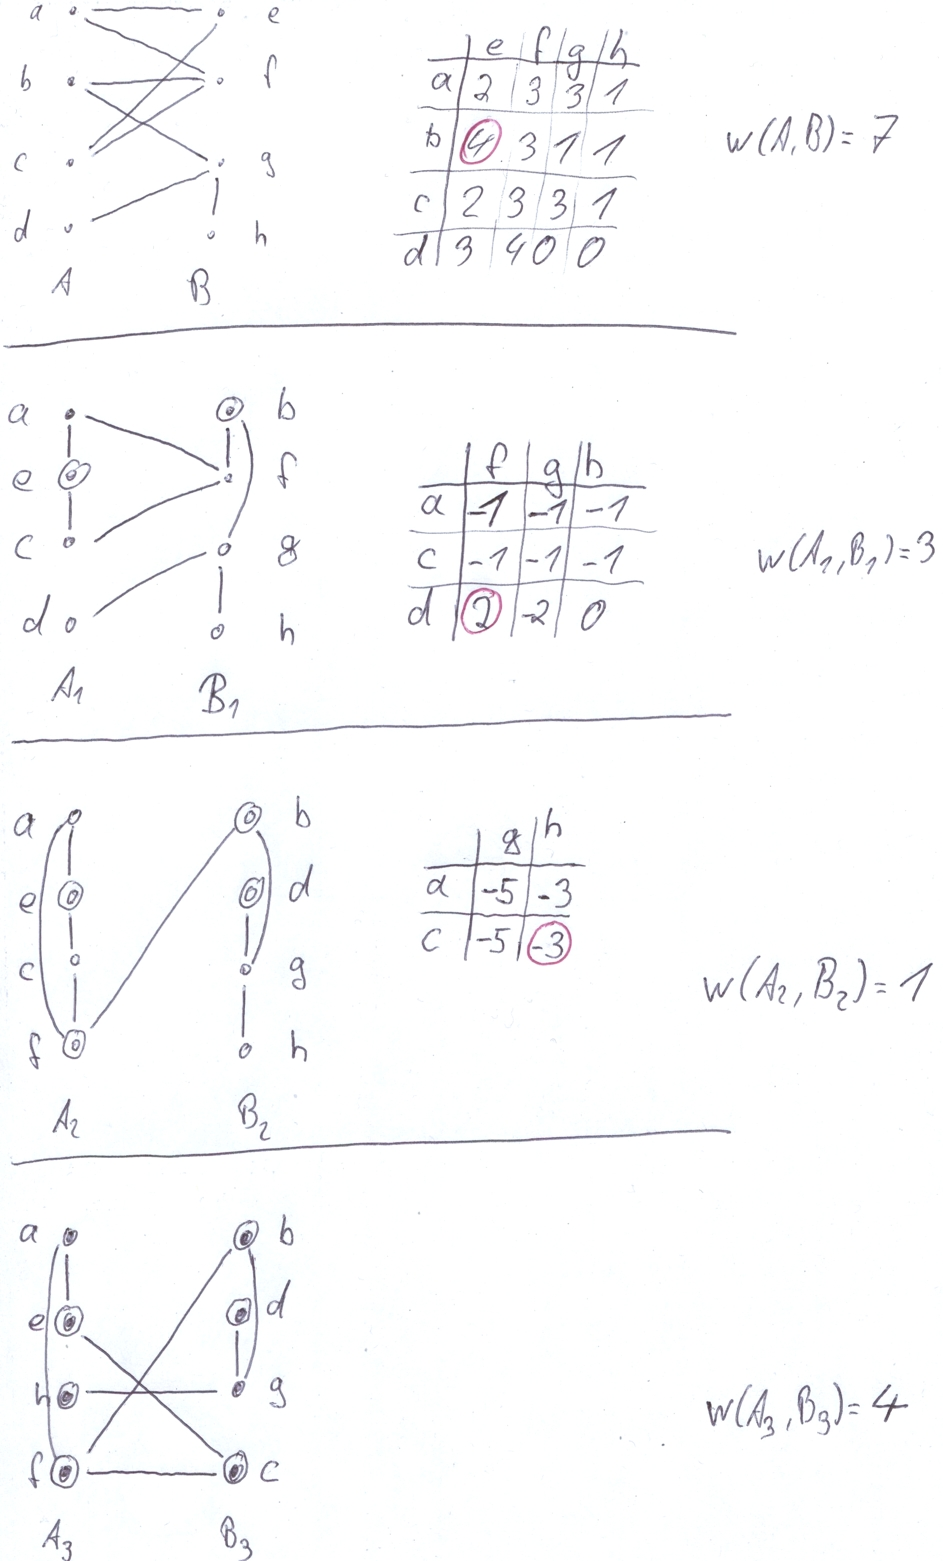
\includegraphics[width=0.9\textwidth]{9_2.jpg}
	\end{figure}

Nach der Erstellung der KL-Nachbarschaft (siehe nächste Seite) von \((A, B)\) würde \((A_2, B_2)\) als neuer Schnitt mit minimalem Gewicht ausgewählt. Im nächsten Schritt der Heuristik würde dann kein besserer Schnitt gefunden werden, da \(w(A_2, B_2)=1\) für einen zusammenhängenden Graphen bereits optimal ist.


\end{document}